\subsection{Know about}

No matter how optimized the representation of the data is and how available we make it, if users are not aware
 of the existence of the resource, they can not use it.

\subsubsection{How to solve it} 
The best way is to advertise the product in the right media with right format.
\subsubsection{How we solve it. Aire Guru} 
Our tool is implemented for the city of Málaga, so we are currently working to publicize it in this city.
It is currently available in the open data portal in the web site tab (https://datosabiertos.malaga.eu/aplicaciones) \\
Aire Guru participated in the first open data reuse contest organized by the Málaga City Council (http://cemi.malaga.eu/es/novedades/detalle/1-Concurso-de-Reutilizacion-de-Datos-Abiertos-del-Ayuntamiento-de-Malaga)
and was a finalist in the web page category.


\begin{figure}[ht]
    \centering
   \subfigure[Advertising in the open data portal of Málaga]{ \centering 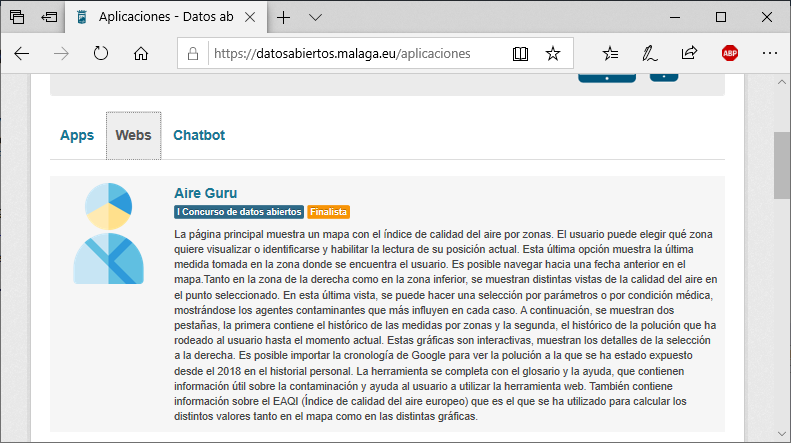
\includegraphics[width=6cm]{aireGuruFinalist}}
   \hfill
   \subfigure[Finalist]{ \centering 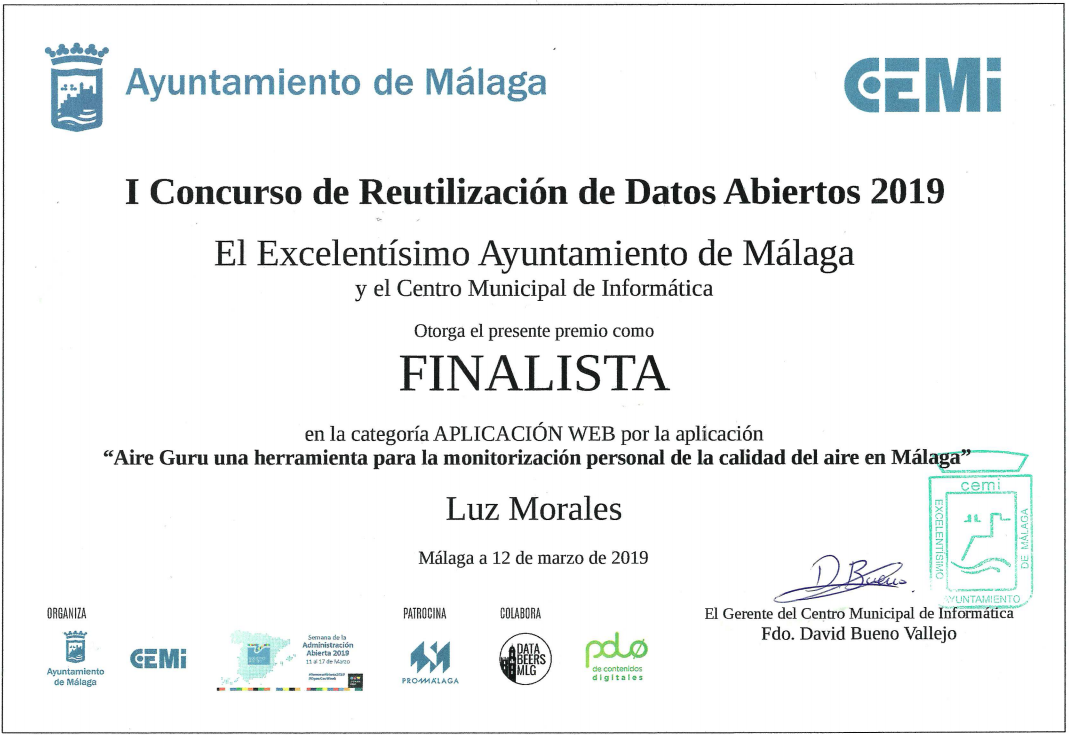
\includegraphics[width=5cm]{aireGuruFinalistCertificate}}
 
    \caption{I Contest of reuse of open data. Málaga's town hall}
    \end{figure}

\elsparagraph{Evaluation}  
\begin{itemize}
    \done It is currently published in the open data portal of the City of Málaga.
\crossed More work should be done on advertising the platform and making it known.
\end{itemize}
\newpage